%\documentclass[a4paper,10pt]{article}
\documentclass[10pt]{article}
\usepackage[utf8]{inputenc}
\usepackage{xspace}
\usepackage{url}
\usepackage{graphicx,graphics} 
\usepackage{color}
\usepackage{amsmath}
\usepackage{amsfonts}
\usepackage{amssymb}
\usepackage{amsthm}
\usepackage{algorithm}
\usepackage{algorithmic}
\usepackage{longtable}
\usepackage{complexity}
\usepackage{tkz-graph}
\usepackage{float}
\usepackage{tabularx}
\usepackage{setspace}
\usepackage{icomma}
\renewcommand{\algorithmicrequire}{\textbf{Input:}}
\renewcommand{\algorithmicensure}{\textbf{Output:}}
\usepackage{authblk}
\usepackage[colorlinks=true,breaklinks=true,linkcolor=blue]{hyperref}


\newcommand\rmatching{${\cal R}$-matching\xspace}
\newcommand\mdelay{$\cal M$-delay\xspace}
\newcommand\matchedgraph{{\bf matched graph}}
\newtheorem{proposition}{Proposition}
\newtheorem{theorem}{Theorem}

\setlength{\parskip}{1ex} % Espace entre les paragraphes

\newtheorem{fact}{Fact}
\newtheorem{lemma}[theorem]{Lemma}
\newtheorem{definition}{Definition}
\newtheorem{corollary}{Corollary}

% \renewcommand{\thefootnote}{\*}

\newcommand{\todo}[1]{{\color{red} TODO: {#1}}}
\newcommand\pazl{\textsc{pazl}\xspace}
\newcommand\pall{\textsc{pall}\xspace}
\newcommand\bra{\textsc{bra}\xspace}
\newcommand\pra{\textsc{pra}\xspace}
\newcommand\minpra{\textsc{min-pra}\xspace}
%opening
\title{Deterministic Scheduling of Periodic Messages for Cloud RAN}
 

\author[1]{Dominique Barth}
\author[1,2]{Ma\"el Guiraud}
% \author[1]{Christian Cad\'er\'e}
 \author[2]{Brice Leclerc}
 \author[2]{Olivier Marc\'e}
\author[1]{Yann Strozecki}
\affil[1]{David Laboratory, UVSQ}
\affil[2]{Nokia Bell Labs France}

\begin{document}
We define by {\bf delay} of a datagram $d$ in a node $u_i$ of a route $r$, the time taken by the datagram to go from $u_0$, the first vertex of the route to $u_i$ through $r$. It is then equal to $DL(d,u_i,r) = t(d,u_j,r) - t(d,u_0,r)$. 
 Thus, the delay of a datagram in the node $u_i$ is equal to $DL(d,u_i,r) =  t(d,u_i,r) - t(d,u_0,r) = \lambda(u_i,r) + \sum_{k=0}^{i-1}( b(d,u_k) + l(d,u_k,r))$.
This delay is composed of three factors:
\begin{enumerate}
\item $\lambda(u_i,r)$ : it is the {\bf physical delay} of the route. This time is not reducible. 
\item  $\sum_{k=0}^{i-1} b(d,u_k)$ : those values correspond to some {\bf physical buffers } induced by the potential speedup or slowdown of the different links of the route used.
\item $\sum_{k=0}^{i-1} l(d,u_k,r)$: are the {\bf logical buffers}, chosen by the solution proposed to solve the problem. Those buffers allows us to control the traffic in every node, and thus, ensure a better QoS of the network.
\end{enumerate}

As a reminder, a stream is a sequence of datagram. Each period, the same sequence of datagrams is sent on a route, in the same order. Let us call $d_0^1$ and $d_1^1$ the two firsts datagram of a stream sent during the first period, and $d_0^2$ and $d_1^2$ the same pair of datagram, sent during the next period. We say that two datagrams $d_i^j$ and $d_i^k$ are associated. Indeed, it correspond to the same datagram but in another period.

The {\bf IP packet delay variation (ipdv) }\cite{demichelis_ip_nodate} is the variation of the delay between two datagram. In our study, we allow some datagrams to be buffered in some nodes of the route, thus, the ipdv between $d_0^1$ and $d_1^1$ can be greater than $0$. Formally, we denote the packet delay variation between two datagrams $d_0^1$ and $d_1^1$ in a node $u$ on a route $r$ by $ipdv(d_0^1,d_1^1,u,r) = |DL(d_0^1,u,r) - DL(d_1^1,u,r) | \ge 0$. 

Note that the ipdv between two associated datagrams is always equal to zero, since the logical delays are deterministic, computed on a period and then applied to all the next periods.

\centering
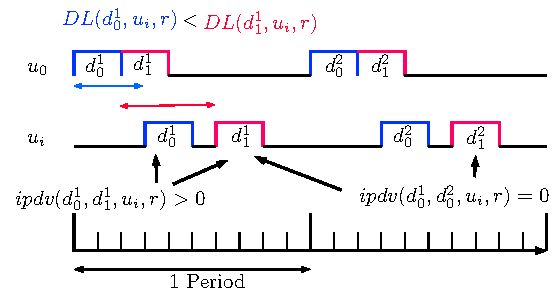
\includegraphics[width=0.8\textwidth]{ipdv}
  
Let us introduce the notion of {\bf jitter} \cite{guillemin_peak_1992} , which commonly correspond to the difference between the minimal and maximal packet delay variation of a datagram in a node. In our case, we introduce some jitters with the logical buffers, that helps to control the network traffic, but since the goal is to reduce the delay of the messages, one can imagine that good deterministic solution will have some low jitters values.

\bibliographystyle{ieeetr}
\bibliography{srcs}

\end{document}
